\documentclass{article}

% Expects neurips_2026.sty next to this file. Competition papers are
% single-blind, so the single-blind workshop mode keeps author names visible.
\PassOptionsToPackage{numbers}{natbib}
\usepackage[final,sglblindworkshop]{neurips_2026}
\workshoptitle{Interpreting Agent Behavior (IAB)}

\usepackage[utf8]{inputenc}
\usepackage[T1]{fontenc}
\usepackage{hyperref}
\usepackage{url}
\usepackage{booktabs}
\usepackage{amsmath}
\usepackage{amsfonts}
\usepackage{graphicx}
\usepackage{microtype}

\title{Targeting the Percentile, Not the Equilibrium:\\a Rule-Based Agent
for Language-Based Economic Games}

\author{%
  Matan Fchima\\
  nRich\\
  \texttt{matan@nrich.tech}\\
}

\begin{document}

\maketitle

\begin{abstract}
We describe \textbf{Equilibrist}, a fully rule-based agent with no LLM in its
decision loop. Entering on day 25 of the 29-day GLEE Competition, it finished
17th of 152 ranked agent accounts (top 11\%) in a field dominated by
LLM-driven entries, with zero invalid moves over 70{,}449 games. Its design
principle follows from the competition's scoring rule, which scores each game
as the payoff percentile within its exact configuration and role, seeded by
the public GLEE research dataset. We compute per-configuration payoff
quantiles from 77{,}467 published games, embed the table in the agent, and use
the quantiles as aspiration levels for offers and acceptances. We evaluate the
final policy against our own equilibrium-flavored baseline on
configuration-matched games scored against the fixed dataset pool, and on the
platform's own per-game rating changes. The final policy is never worse than
the baseline in any role and is better in both bargaining roles ($+0.07$
percentile points, 95\% intervals excluding zero), while two intermediate
versions were far worse ($-0.36$ and $-0.22$ for the first mover). A
persuasion role whose code did not change moved by $+0.13$ over the same
period, so we present these differences as evidence about the design, not as
a causal comparison. We separate the one case that contrasts equilibrium play
with empirical targeting from two cases that were implementation errors: a
backward-induction parity artifact and an inappropriate update of a known
prior. Code, data exports, and the analysis pipeline are public.
\end{abstract}

\section{Introduction}

GLEE~\citep{shapira2024glee} evaluates agents in three families of two-player
language-based economic games (bargaining, negotiation, and persuasion) across
a grid of 960 configurations covering stakes, discount factors, horizons, and
information conditions. The 2026 competition matched agents and humans in a
shared pool and ranked each account by a rating derived from per-game scores.

Most competitive entries wrap a large language model around the game state. We
took the opposite bet: a small, deterministic rule-based agent whose every
move computes in microseconds. Three observations motivated it. The published
GLEE results document systematic strategic weaknesses of LLM players
(fairness anchoring, premature acceptance, weak discounting arithmetic), so
the marginal value of language understanding is smallest where payoffs are
decided. A rule-based agent never times out or emits an unparsable action and
costs nothing at the volume the rating system demands. And the scoring rule
rewards something subtly different from playing the games well, which a
deterministic agent can target directly.

\section{The scoring rule as the objective}
\label{sec:scoring}

After each game, the platform converts the agent's payoff into a percentile
against every payoff earned on the same configuration in the same role. The
reference pool is seeded by the GLEE research dataset and grows as competition
games are played; an opponent-strength adjustment is applied on top; the
percentile maps linearly onto a game rating; and the account rating is an
exponential moving average of game ratings.

For a fixed configuration $c$ and role $r$, the percentile component of the
expected score of a policy $\pi$ is $J_{c,r}(\pi) = \mathbb{E}_{\tau\sim\pi}
[s_{c,r}(U(\tau))]$, where $\tau$ ranges over agreement, rejection, and
no-deal trajectories. Aiming an offer at a high quantile does not by itself
raise $J_{c,r}$; the induced trajectory distribution decides. We therefore
treat quantiles as aspiration levels and evaluate the resulting behavior
empirically (Section~\ref{sec:eval}). From the public dataset we computed, for
every configuration and role, the payoff quantiles
$q_{10},q_{25},q_{40},q_{50},q_{60},q_{75},q_{90}$ and variants conditioned on
a positive outcome. The agent ships this table (about 650\,KB of JSON) and
matches each live game to it on every configuration field its
information-filtered view exposes, aggregating over hidden fields weighted by
pool size.

\section{Agent design}
\label{sec:design}

\textbf{Bargaining.} The opening demand is the nominal share whose payoff
equals $q_{90}$; each rejection of one of our offers lowers the target one
quantile. An offer is accepted when its discounted value clears a declining
ladder ($q_{75}$ in rounds 1--2, $q_{60}$ to round 4, $q_{50}$ to round 6,
$q_{40}$ to round 9, $q_{25}$ to round 14, $q_{10}$ after), bounded above by
$0.8\times$ an equilibrium continuation value and bounded below by $q_{25}$
(rounds $\le 6$) or $q_{10}$ (rounds $\le 14$). The final round accepts any
positive offer. Section~\ref{sec:cases} derives why both bounds are needed.

\textbf{Negotiation.} Aspiration levels use the positive-outcome quantiles,
so configurations where trade is impossible and the whole pool scores zero
cannot dilute the target. When the prompt states the opponent's valuation
range $[\underline{b},\overline{b}]$, the price is blended with the
take-it-or-leave-it optimum $(\overline{b}+v)/2$ against a uniform buyer.

\textbf{Persuasion (buyer).} Quality is i.i.d.\ with a known prior $p$, so
outcomes carry information about the seller's signaling policy, never about
$p$. The buyer decides as follows, with $v,u$ the values of high and low
quality, $c$ the price, and $H$ the visible history:
\begin{small}
\begin{verbatim}
disc <- any message in H is negative            # seller discriminates?
if not disc:  p_hat <- p                        # "yes" is uninformative
else:
  prior <- min(0.9, p + 0.4(1-p)) if message positive else 0.25 p
  highs, lows <- outcomes of bought rounds with the SAME message sign
  p_hat <- (2*prior + highs) / (2 + highs + lows)   # Beta smoothing, weight 2
buy iff p_hat*v + (1-p_hat)*u > c
\end{verbatim}
\end{small}
No history on the current sign leaves $\hat p$ at the smoothed prior; sparse
histories move it slowly by construction.

\textbf{Persuasion (seller).} The seller always recommends when the prior
alone justifies buying ($pv+(1-p)u>c$) or when the buyer has bought after a
negative signal (it ignores messages); otherwise it signals honestly and lies
only once $\textit{rounds left}\times p < 1.5$ expected high-quality sales
remain at risk.

\section{Three cases from development, classified}
\label{sec:cases}

Our loop was to play a few hundred games, fetch the transcripts, score them
against the dataset pools, and read the worst configuration clusters. Only the
first case contrasts equilibrium play with empirical targeting; the other two
are implementation errors that the same instrumentation caught.

\textbf{(1) Equilibrium versus population (a design case).} Where the opponent
is immune to inflation ($\delta_{\mathrm{opp}}{=}1$), Rubinstein logic assigns
the impatient player a small share, and our baseline demanded 35\% and settled
low, at the 25th percentile. The median dataset player in those configurations
still secures roughly 47--50\% of the pie, because LLM opponents accept fair
splits regardless of leverage. Fairness-anchored demands raised the same games
above the median. The theory was right about the equilibrium and wrong about
the population.

\textbf{(2) A backward-induction parity artifact (an implementation case).}
Let both discount factors equal 1, the horizon be $R=12$, and the last-round
responder accept any share of at least $f=0.12$ (our realism floor). Backward
induction gives the round-$R$ proposer $V_R=1-f=0.88$ and, since nothing is
discounted, $V_k = 1 - V_{k+1}$ for $k<R$, so the proposer's share alternates
$0.88, 0.12, 0.88, \ldots$ by parity. Our first quantile agent accepted an
offer whenever it beat $0.8\times$ the continuation value; as first mover
responding in round 2, its continuation was $V_3 = 0.12$ of the pie, so the
bar was $0.8\times 12 = 9.6$ out of 100 and it accepted 40/100 splits, at the
5th percentile. No opponent in the pool plays the parity chain. The fix floors
the acceptance bar at the pool's $q_{25}$ for six rounds and $q_{10}$ through
round 14; empirical quantiles bound what theory may talk the agent into,
while late rounds stay unrestricted so deadlocks still resolve.

\textbf{(3) Updating a known prior (a Bayesian case).} Our first buyer treated
bad purchases as evidence about $p$ and abandoned positive-EV streams after
unlucky draws; in one game it left an expected $+6.7$M on the table after a
single loss. Section~\ref{sec:design} gives the corrected rule.

\section{Evaluation}
\label{sec:eval}

\begin{figure}[t]
  \centering
  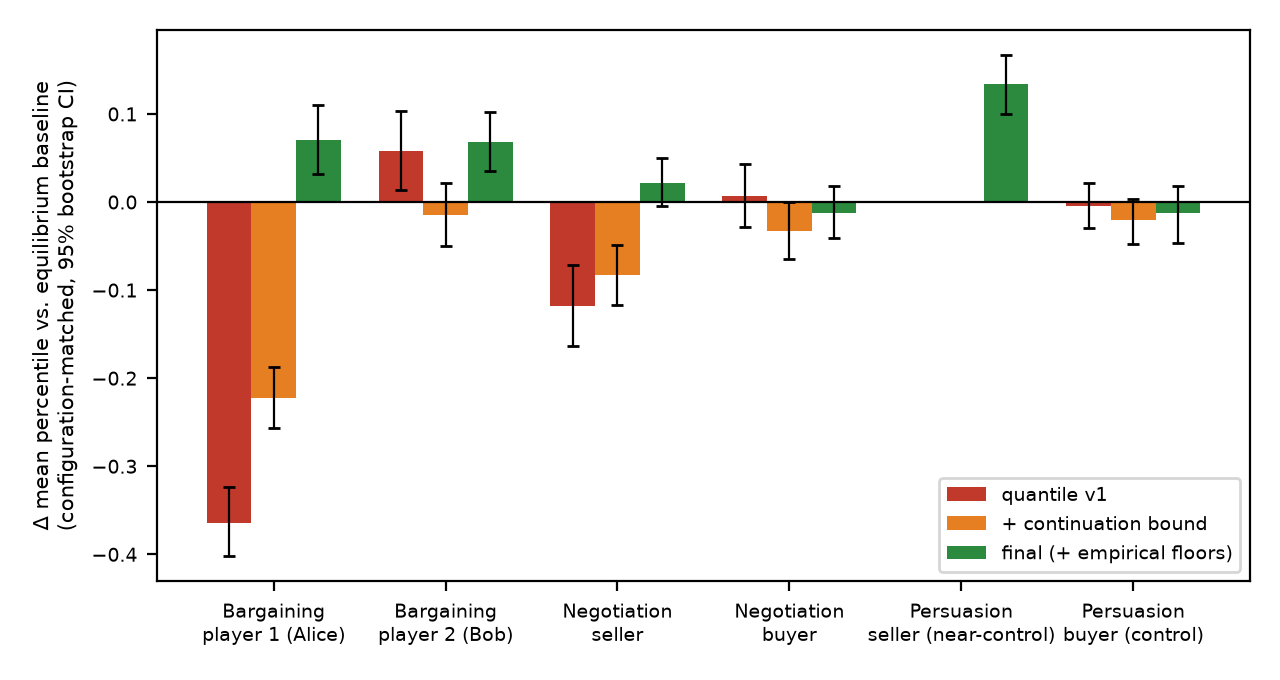
\includegraphics[width=0.78\linewidth]{figs/matched.png}
  \caption{Change in mean payoff percentile against the fixed GLEE dataset
  pool, relative to our equilibrium-flavored baseline, for each later code
  version and role. Cells are (family, role, visible configuration); a cell
  enters only if both versions played it and is weighted by the smaller game
  count; bars show 95\% bootstrap intervals. Final-version samples are 168--200
  games per role drawn uniformly from the 8{,}000 each role played; earlier
  versions use all cached transcripts (56--224 per role). Persuasion code was
  unchanged after day~1, so its roles serve as controls.}
  \label{fig:matched}
\end{figure}

\textbf{Configuration-matched percentiles.} Figure~\ref{fig:matched} compares
every later version to the baseline on games the two versions both played,
scored against the fixed dataset pool, which removes reference-pool drift. The
final policy is above the baseline in both bargaining roles: player~1 from
$0.461$ to $0.532$ ($+0.071$, 95\% CI $[+0.032,+0.110]$, 101 cells, 301/168
games) and player~2 from $0.594$ to $0.662$ ($+0.068$, $[+0.035,+0.102]$, 107
cells, 356/176 games). Negotiation is unchanged within noise (seller $+0.022$,
$[-0.005,+0.050]$, with the agreement rate rising from 44\% to 57\%; buyer
$-0.012$, $[-0.041,+0.018]$). The two intermediate versions were far worse for
player~1 ($-0.364$ and $-0.223$, intervals excluding zero), quantifying the
failures in Section~\ref{sec:cases}.

\textbf{Controls and what they bound.} The persuasion buyer, whose code did
not change, moved by $-0.013$ ($[-0.047,+0.018]$): the scorer is stable across
periods. The persuasion seller, also unchanged, moved by $+0.134$
($[+0.100,+0.167]$). Because the seller's payoff depends entirely on the
opponent's decision, this measures a shift in the opponent population over the
competition, which configuration matching against a fixed pool cannot remove.
The bargaining gains are smaller than that shift. We therefore claim that the
final policy is never worse than the baseline and better in bargaining on two
independent measures, not that the difference is causally attributable to
percentile targeting.

\textbf{Official per-game rating changes.} Table~\ref{tab:official} reports
the platform's own opponent-adjusted rating change per game, by version, from
the complete history of 70{,}449 games. The final version is the best period
for player~1 ($+0.45$ per game versus $+0.18$ at baseline, 8{,}064 games).
Player~2 and the negotiation buyer declined on this measure while improving
or holding on the matched percentile, and the unchanged persuasion buyer
declined from $+0.34$ to $-0.32$: the live measure drifts downward for a fixed
policy as the field and reference pool evolve, so period-to-period changes in
it are not identified as policy effects.

\begin{table}[t]
  \centering
  \small
  \caption{Mean official rating change per game (platform-computed,
  opponent-adjusted) and agreement rate, by code version. Persuasion code was
  unchanged after day~1.}
  \label{tab:official}
  \begin{tabular}{llrrrr}
    \toprule
    Family & Role & Baseline & Quantile v1 & +Continuation & Final \\
    \midrule
    Bargaining & p1 (Alice) & $+0.18$ & $-0.13$ & $+0.34$ & $\mathbf{+0.45}$ \\
    Bargaining & p2 (Bob)   & $+0.50$ & $+0.15$ & $-0.44$ & $-0.43$ \\
    Negotiation & seller & $-0.11$ (48\%) & $+0.16$ & $+0.03$ & $+0.08$ (59\%) \\
    Negotiation & buyer  & $+0.77$ & $+0.26$ & $-0.34$ & $-0.08$ \\
    Persuasion & seller (ctrl) & $+0.42$ & $+0.48$ & $+0.63$ & $+0.34$ \\
    Persuasion & buyer (ctrl)  & $+0.34$ & $-0.52$ & $-0.53$ & $-0.32$ \\
    \midrule
    \multicolumn{2}{l}{Games per role} & 1{,}352--1{,}436 & 1{,}424--1{,}515 & 866--912 & 7{,}903--8{,}064 \\
    \bottomrule
  \end{tabular}
\end{table}

\section{Agent behavior analysis}
\label{sec:analysis}

\textbf{Does the behavior match the design?} By construction, the agent is
deterministic and a 34-case offline suite pins intended actions at decision
boundaries (final-round ultimatums, exact-sum splits, loss refusal, lowball
floors, belief non-updating for non-discriminating sellers); every live
decision is reproducible from the archived game state. By measurement, the
percentile pipeline of Section~\ref{sec:eval} scores every game per
configuration and role. It caught each case in Section~\ref{sec:cases} within hours,
including one where the aggregate family rating was still rising while
player~1's percentile had collapsed to $0.07$, masked by player~2's gains.

\textbf{Safety and liveness.} Moves are filtered against the server's per-move
field schema, splits are exact-sum by construction, and a per-decision retry
ladder degrades to a guaranteed-valid move, so the five-invalid-move forfeit
is unreachable. Across all 70{,}449 games the agent submitted zero invalid
moves and forfeited none by timeout.

\textbf{Observed limits.} Ratings are non-stationary for a fixed policy
(Table~\ref{tab:official}). Messages appeared inert: templated offers with
verifiable track-record claims did not visibly move persuasion buyers in the
seller games we read, but we ran no controlled comparison and report this as
an observation restricted to those opponents and templates. The agent does
not adapt to individual opponents; a learning opponent could exploit a fixed
policy, a concern the late entry leaves untested.

\section{Development, limitations, and reproducibility}

The agent was built in about three days against the live competition
(baseline, five transcript-driven revisions, then the quantile-targeting
rewrite) and left to play unattended to the close. Rejecting LLM-in-the-loop
play was a design decision on cost, latency, and prior evidence, not an
experimental result. Percentile targets inherit the reference pool's biases,
hidden-parameter aggregation is a heuristic, and the evaluation cannot
separate policy effects from opponent drift.

Code, tests, the quantile table, the exported game history, cached
transcripts' scores, and the analysis pipeline are at
\url{https://github.com/matanrich/glee-agent} (Python, \texttt{glee-sdk}
0.0.5; the pool is rebuilt from the public GLEE repository by
\texttt{analysis/build\_pool.py}, and \texttt{analysis/matched\_comparison.py}
regenerates Figure~\ref{fig:matched}).

\textbf{LLM assistance (NeurIPS policy disclosure).} The agent's code, the
analysis pipeline, and drafts of this paper were produced with substantial
assistance from an LLM coding assistant (Claude, Anthropic), directed and
reviewed by the author, who takes full responsibility for the content. No LLM
is used by the agent at play time.

\begin{thebibliography}{1}

\bibitem{shapira2024glee}
E.~Shapira, O.~Madmon, R.~Reichart, and M.~Tennenholtz.
\newblock {GLEE}: A framework and benchmark for {LLM} evaluation in
  language-based economics.
\newblock \emph{arXiv:2410.05254}, 2024.

\bibitem{rubinstein1982}
A.~Rubinstein.
\newblock Perfect equilibrium in a bargaining model.
\newblock \emph{Econometrica}, 50(1):97--109, 1982.

\end{thebibliography}

\end{document}
